\section{Computation with Incomplete Information}
\subsection{Overview}
\begin{figure}
  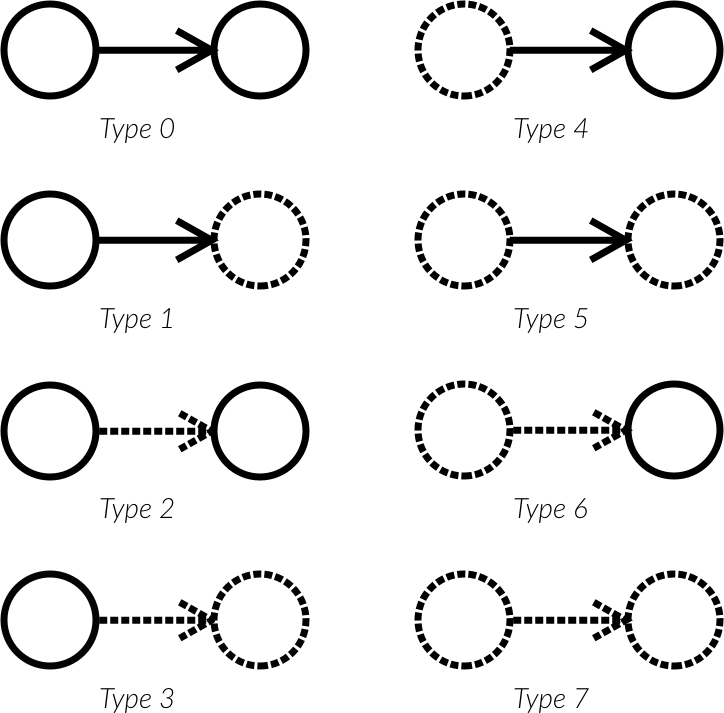
\includegraphics[width=\linewidth]{img/types.png}
  \caption{All Possible Types of Incomplete Computation}
  \label{fig:types}
\end{figure}

The name system is using binary numbering, where the dashed objects are 1s and the solid ones are 0s. For example, Type 3 is 011, which in binary is 3.

As we can assume that Turing machine is the foundation of all. Then, we have to be able to define things which is distinguishable. So here are all the distinguishable parts

The Type 0 is a complete fact that we have all the input, the instruction and the output. The Type 1 is simply the normal computation. Nothing fancy about Type 1. All the programs we all running is Type 1.

Type 2 is when we don't know what exactly is the transformation rules. In this case, we are dealing with physics and science, where we know input and output and guess what't the governing rules underneath. We can't 100\% sure about the result, all we can know is that for some sense we can't distinguish the rules underneath and the rule we present at a certain level. While we mean learning, this is exactly the case.

Type 4 is when we knows the rule and output and guess the input. Here we are doing engineering and solving a searching problem. Also, in this type, we are using it as a sieve or a checker, to define a class, which means we are use type 4 to abstract. Type 4 is as important as type 1, as it's the driven force of reduce the computational cost as we will discuss in chapter 4.

Type 5 is basically the function we write in daily routine programming. Where you using some symbol to denote some operands in the transformation. As we will discuss in chapter 2, the equivalence of computation of Type 5 is one of the core functionality in abstract thinking.

Type 3 is when you don't know the function as well as the output, you only know the input, while in this case, it's like you type $f(3)$, nothing intereting happens here as far as I can see. But if you insist say at least we know the input, then in this case the thing is that you could compute with this information. This will be helpful when we discuss it as solving problems as purposeless transformation.

Type 6 is also boring as type 3, where it's like asking $f(x) = 3$, where you don't know any thing about the function and the input. But the same as Type 5, it will be helpful when we discuss about the inverse implications.

Type 7 is $f(x)$, this would be the highest abstraction we can get, and all the above abstraction can be transform back to this form.

For each type, you can always find a equivalence form of it and also you can combine (or link) them to perform a more complicated thing. And combine and abstract is the common themes.

\subsection{Classification and Abstraction}
\begin{figure}
  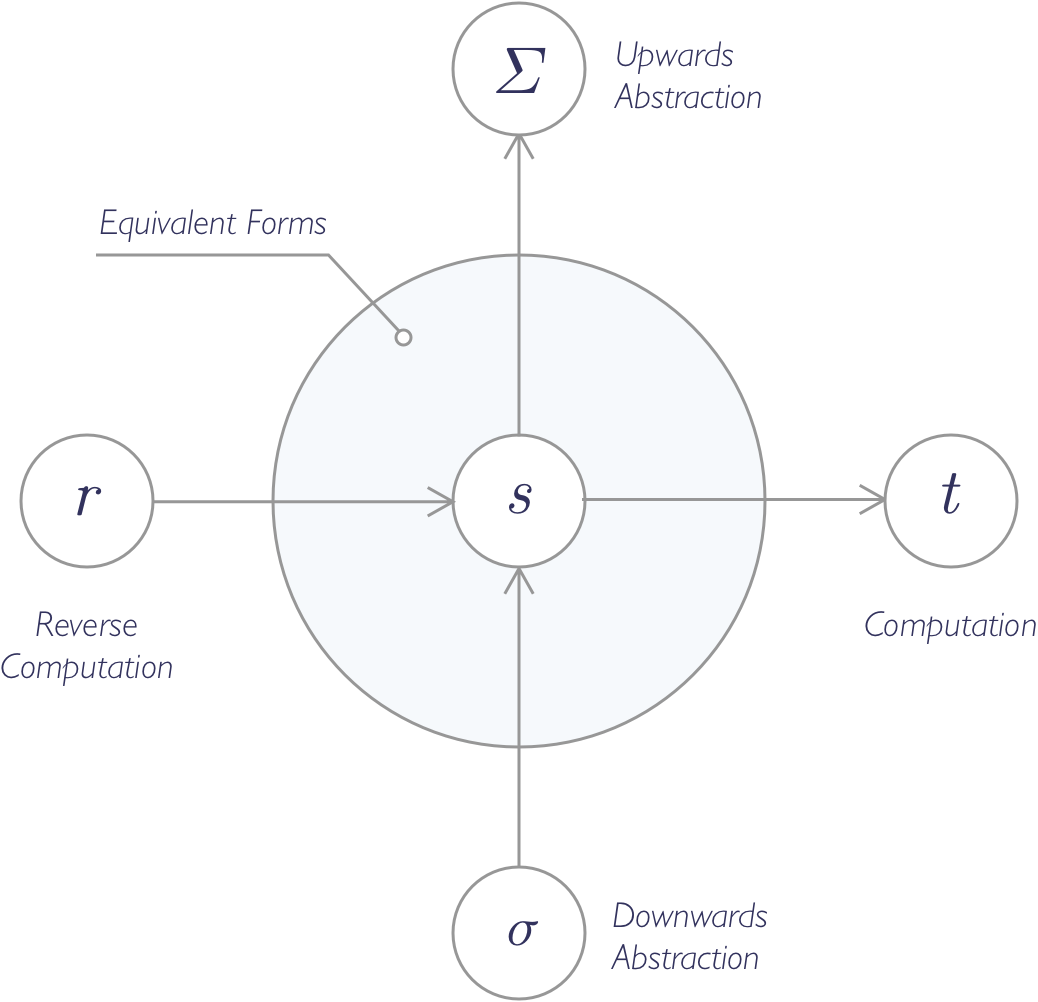
\includegraphics[width=\linewidth]{img/moves.png}
  \caption{All Possible Moves from a Valid Statement}
  \label{fig:moves}
\end{figure}

\subsection{Induction and Learning}
\subsection{Reverse Implications}
\subsection{Symbolic Functions}
% \subsection{Implications}
\subsection{Computational Facts}
\subsection{Combination of Computational Facts}
